\chapter{THE STANDARD MODEL AND SUPERSYMMETRY}
\label{chap:theory}

\section{The standard model of particle physics}
\label{sec:StandardModel}
The standard model (SM) of particle physics is a Lorentz-invariant quantum field theory that describes elementary particles and their allowed interactions
The first piece of the standard model was developed in 1961 with the unification of the electromagnetic and weak interactions 
\cite{GLASHOW1961579,Glashow:1970gm}. 
The Higgs mechanism was incorporated a few years later 
\cite{PhysRev.127.965,PhysRevLett.13.508,PhysRevLett.13.321,Guralnik:1964eu}, and 
the standard model took on the form we know today with the inclusion of the strong force and quantum chromodynamics (QCD) in the 1970's \cite{PhysRevLett.19.1264}.
The standard model is incredibly successful, and it has made absurdly precise predictions that have held up to experimental scrutiny. 

The standard model is a non-Abelian gauge theory. The symmetry group of the standard model is 
\begin{equation}
G_{SM} = SU(3)_C \otimes SU(2)_L \otimes SU(1)_\Upsilon
\label{equ:symm}
\end{equation}
where $SU(3)_C$ is responsible for mixing the 3 \textit{colors} of quarks and antiquarks in QCD, $SU(2)_L$ represents \textit{weak isospin}, and $U(1)_\Upsilon$ couples to the \textit{weak hypercharge $\Upsilon$}. The combination $SU(2)_L \otimes SU(1)_\Upsilon$ corresponds to the electroweak interactions. 

%%%%%%%%%%%%%%%%%%%%%%%%%%%%%%%%%%%%%%%
\subsection{Particle content of the standard model}
\label{sec:SMparts}
The fields in the SM are identified by their representation in the symmetry group of Equation~\ref{equ:symm}. These are listed for the SM fermions in Table~\ref{tab:fermions} and for the gauge bosons in Table~\ref{tab:bosons}. There are three generations of quarks and three generations of leptons in the SM. The quarks are in a non-trivial representation of all three SM symmetries, and therefore interact via the strong, weak, and electromagnetic interactions. The three ``up-type" quarks are the up quark $u$, the charm quark $c$, and the top quark $t$. The three ``down-type" quarks are the down quark $d$, the strange quark $s$, and the bottom quark $b$. 

The three generations of leptons include the electron $e$, muon $\mu$, and tau $\tau$ and the corresponding neutrinos. In the SM, the neutrinos are massless, even though it has been experimentally established that at least two of the neutrinos must have non-zero mass 
\cite{PhysRevLett.81.1562,PhysRevLett.87.071301,PhysRevLett.89.011301}. 
The electron, muon and tau particles participate in the weak interaction and the electromagnetic interaction, but the neutrinos, being electromagnetically neutral, only participate in the weak interaction. 

As can be seen in Table~\ref{tab:fermions}, the weak interaction does not respect parity. The left-handed quarks and leptons belong to $SU(2)_L$ doublets, whereas the right-handed quarks and leptons form $SU(2)_L$ singlets.

\begin{table}[ht]
    \caption{FERMIONS IN THE STANDARD MODEL}
    \centering
    \begin{tabular}{|c|c|c|c|}
    \hline
    \hline
    Name  & Symbol & $SU(3)_C,~SU(2)_L,~U(1)_\Upsilon $\\
  	  \hline
           \hline    
quarks        & ($u_L~d_L$)     & (\textbf{3}, \textbf{2}, $\frac{1}{6}$) \\
(3 families) & $u_R^\dagger$ & ($\bar{\textbf{3}}$, \textbf{1}, $-\frac{2}{3}$) \\
                   & $d_R^\dagger$ & ($\bar{\textbf{3}}$, \textbf{1}, $\frac{1}{3}$) \\
                   \hline
leptons       & ($\nu~e_L$)      &  (\textbf{1}, \textbf{2}, $-\frac{1}{2}$) \\
(3 families) & $e_R^\dagger$ &  (\textbf{1}, \textbf{1}, 1) \\
           \hline
           \hline
    \end{tabular}
    \label{tab:fermions}
    \justify{Fermions in the standard model and their representations under $G_{SM}$. }
\end{table}

%%%%%%%%%%%%%%%%%%%%%%%%%%%%%%%%%%%%%%%
The gauge bosons are responsible for mediating the interactions between the fermions. Before electroweak symmetry breaking (EWSB), the three gauge bosons of $SU(2)_L$ are the $W^+,~W^-,$ and $W^0$, and the $U(1)_\Upsilon$ gauge boson is the $B$ boson. After EWSB, the $W^+$ and $W^-$ bosons gain a mass, and the $W_0$ and $B$ bosons mix to form the massive $Z$ boson and the massless photon $\gamma$. EWSB will be described in more detail in Section~\ref{sec:EWSB}.

For the strong force $SU(3)_C$, the gauge bosons are the gluons. Processes involving the interactions of quarks and gluons are referred to as QCD processes. The QCD interaction is different from the electroweak interactions in that the strong force grows in strength at larger distances. This leads to the phenomenon of \textit{confinement}: at low energies and large distances (greater than ~1 GeV$^{-1}$), we cannot identify individual quarks or gluons. Instead, these particles can only be found in $SU(3)_C$ singlets, typically either mesons ($q\bar{q}$) or baryons ($qqq$ or $\bar{q}\bar{q}\bar{q}$). 

\begin{table}[ht]
    \caption{GAUGE BOSONS IN THE STANDARD MODEL}
    \centering
    \begin{tabular}{|c|c|c|c|}
    \hline
    \hline
    Name  & Symbol & $SU(3)_C,~SU(2)_L,~U(1)_\Upsilon $\\
  	  \hline
           \hline    
gluon         & $g$   & (\textbf{8}, \textbf{1}, 0) \\
\hline
$W$ bosons & $W^\pm,~W^0$ & (\textbf{1}, \textbf{3}, 0) \\
\hline
$B$ boson & $B^0$ & (\textbf{1}, \textbf{1}, 0) \\
           \hline
           \hline
    \end{tabular}
    \label{tab:bosons}
    \justify{Gauge bosons in the standard model before electroweak symmetry breaking and their representations under $G_{SM}$. }
\end{table}

%%%%%%%%%%%%%%%%%%%%%%%%%%%%%%%%%%%%%%%

Finally, the only particle not included in Table~\ref{tab:fermions} or \ref{tab:bosons} is the Higgs boson. The Higgs boson was discovered by the CMS and ATLAS collaborations in 2012 \cite{ATLASHiggs,CMSHiggs}, and is responsible for EWSB. It is the only fundamental scalar in the SM and has a mass of approximately 125 GeV. The Higgs boson is in the (\textbf{1}, \textbf{2}, $+\frac{1}{2}$) representation of $G_{SM}$, and is therefore uncharged under the strong and electromagnetic interactions. 

Figure~\ref{fig:SMint} summarizes the SM particles and their allowed interactions.

\begin{figure*}[htbp]
    \centering
    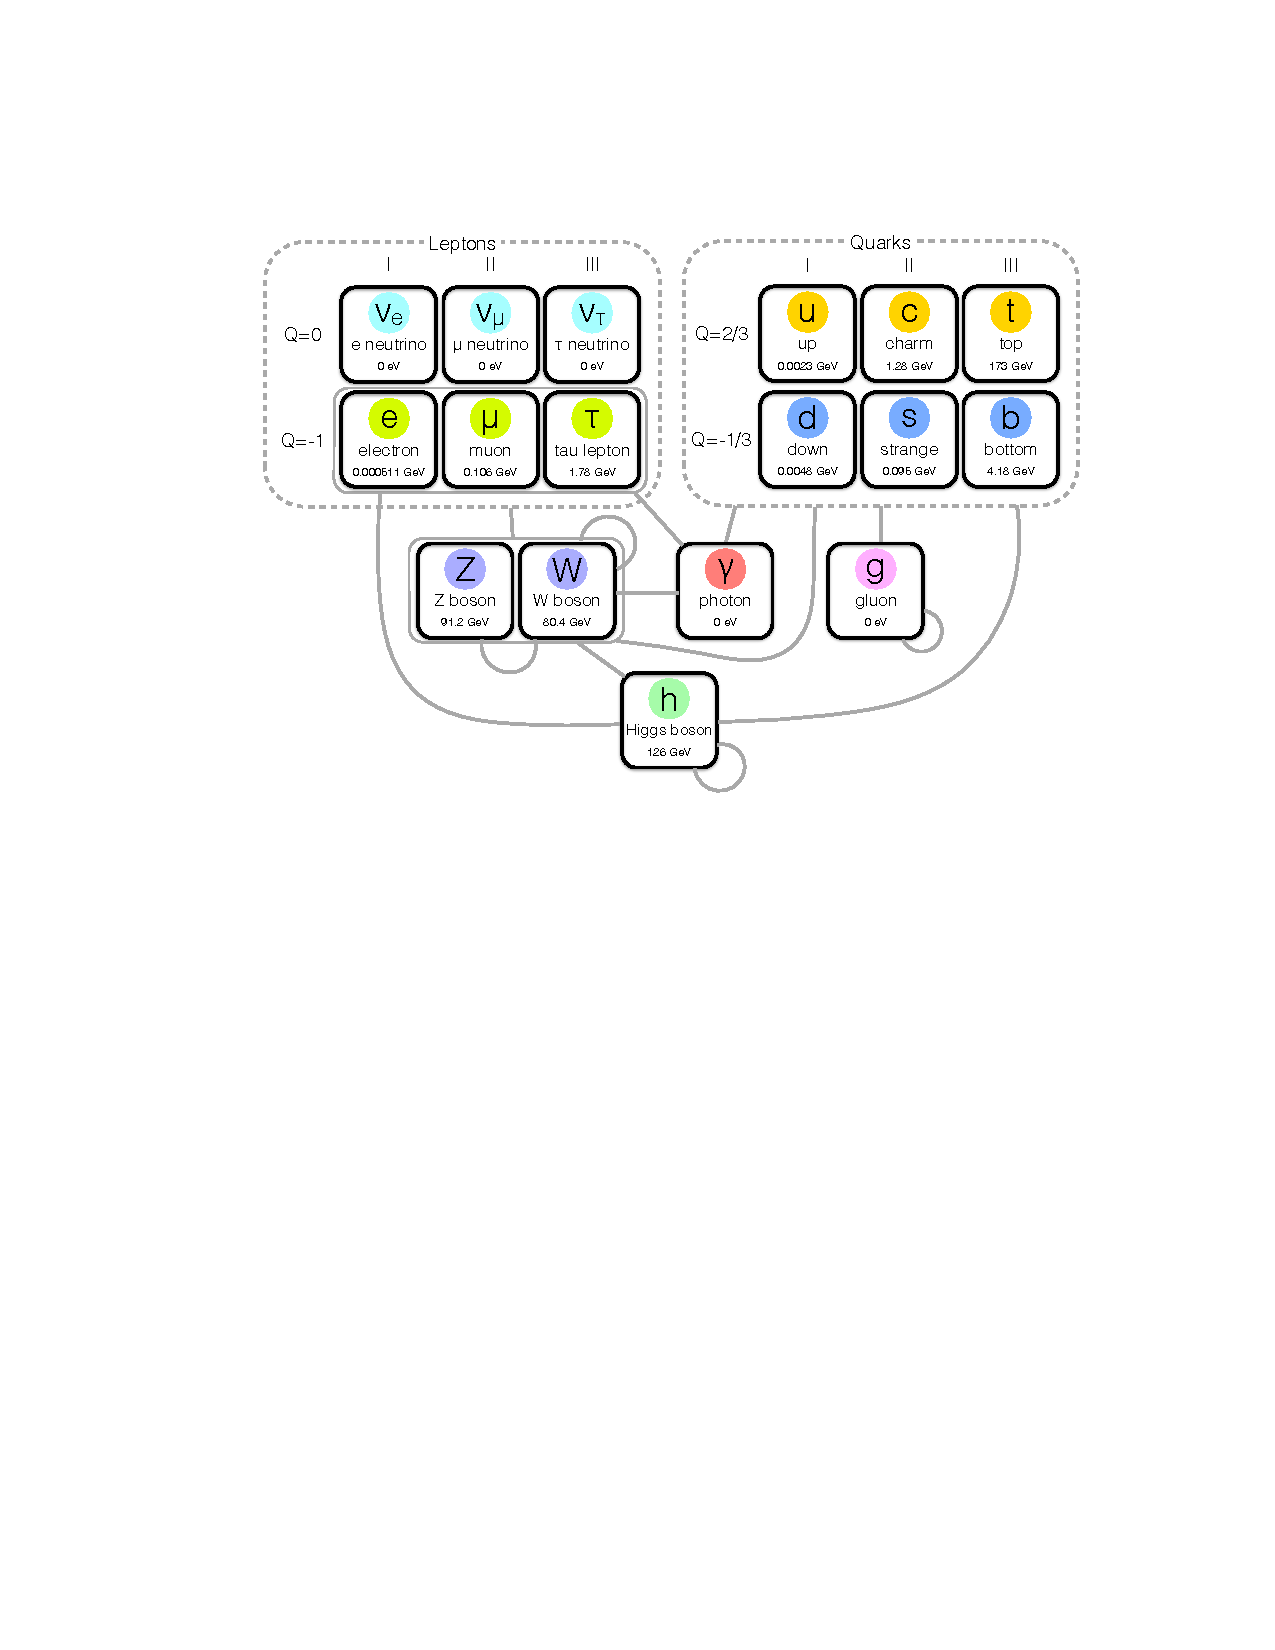
\includegraphics[width=\textwidth]{Figures/Theory/SM_Interactions.pdf}
    \caption{Particle content of the standard model. Allowed interactions are indicated with gray lines between particles or particle groups. The mass of each particle is listed underneath its symbol and name. The electric charge Q of the leptons and quarks is also indicated. Particles connected to themselves can have self-interactions.
    Reprinted from Reference~\cite{Yutaro}.}
    \label{fig:SMint}
\end{figure*}

%%%%%%%%%%%%%%%%%%%%%%%%%%%%%%%%%%%%%%%
%%%%%%%%%%%%%%%%%%%%%%%%%%%%%%%%%%%%%%%

\subsection{Electroweak symmetry breaking}
\label{sec:EWSB}
Electroweak symmetry breaking is a crucial feature of the standard model. The electroweak symmetry is spontaneously broken through the Higgs mechanism. 
The scalar potential of the complex Higgs field $H$ is
\begin{equation}
V(H^\dagger H) =  \mu^2(H^\dagger H) + \lambda(H^\dagger H)^2. 
\label{equ:HiggsV}
\end{equation}

The mass parameter $\mu^2$ is negative, which means that the vacuum expectation value (vev) of the Higgs (written as $\langle H \rangle$ or $v$) is non-zero. The Higgs potential is illustrated in Figure~\ref{fig:HiggsV}. Spontaneous symmetry breaking occurs when the value of the Higgs field ``rolls" from the unstable position at the origin and comes to rest at the stable minima:
\begin{equation}
\langle H \rangle= v = \sqrt{\frac{-\mu^2}{2\lambda}}.
\end{equation}
The value of $v$ has been measured in electroweak interactions to be about 174 Gev. 

\begin{figure*}[htbp]
    \centering
    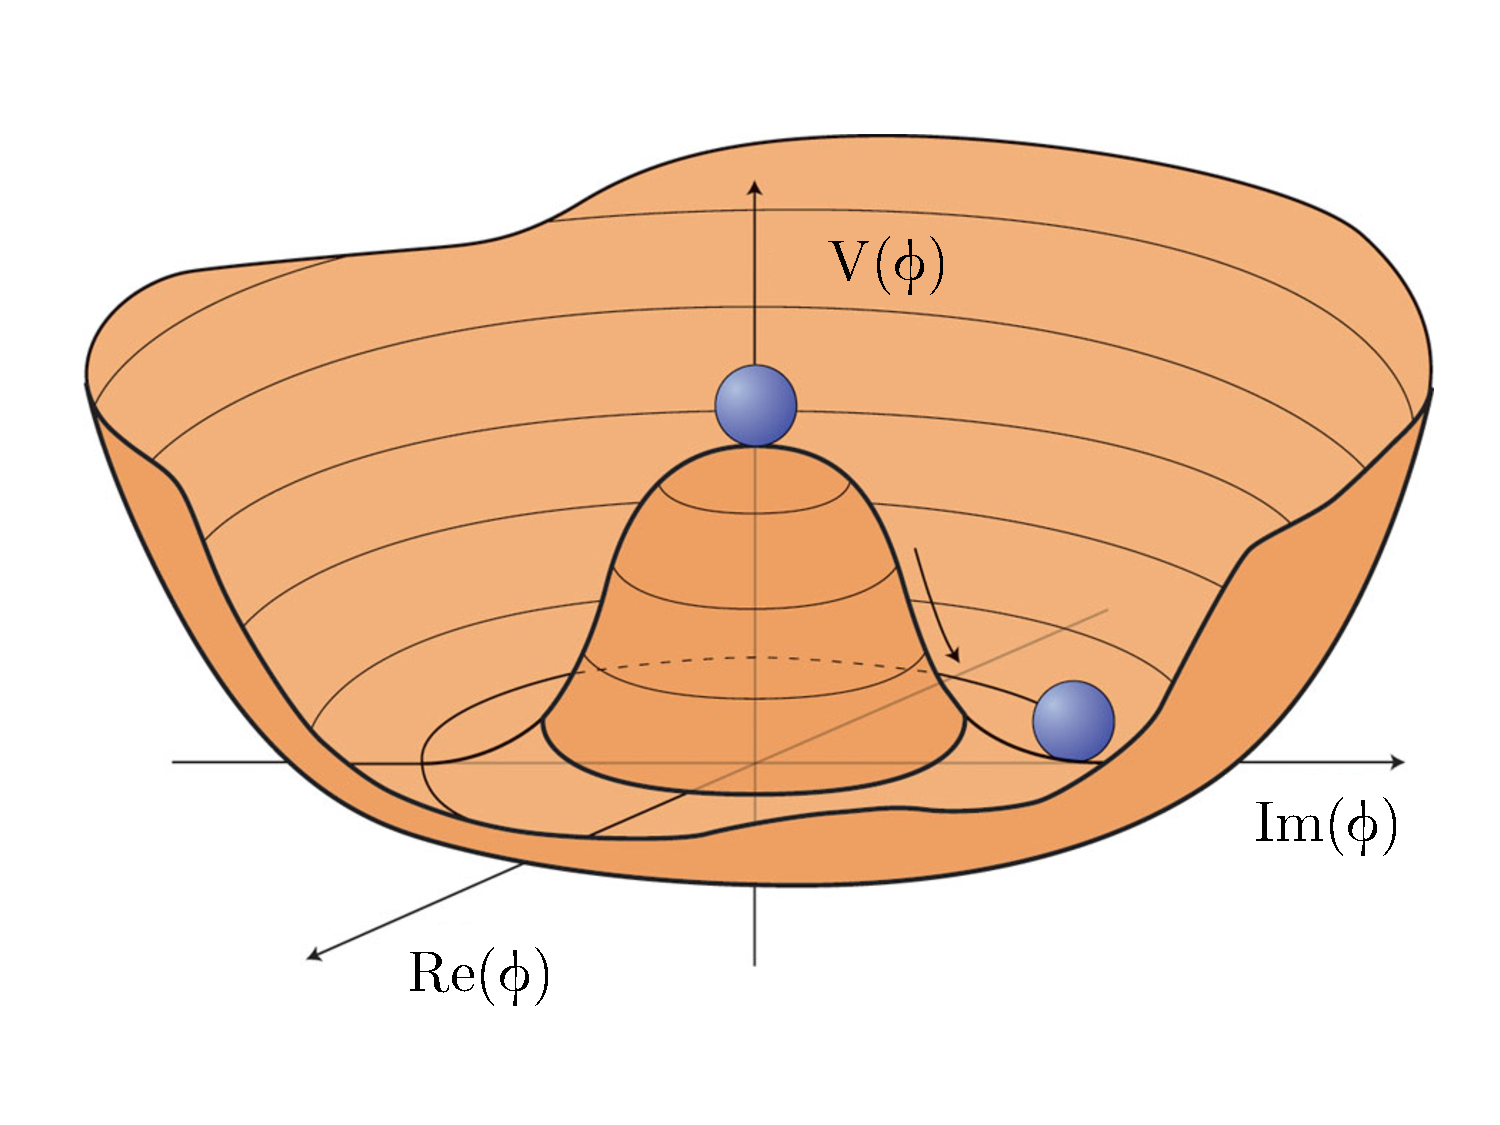
\includegraphics[width=0.8\textwidth]{Figures/Theory/improvedMexicanHat.pdf}
    \caption{Cartoon illustrating the Higgs potential. The Higgs field during spontaneous symmetry breaking can be thought of as the ball, which ``rolls" from the unstable point to the stable minima.
    Reprinted from Reference~\cite{mexicanHat}.}
    \label{fig:HiggsV}
\end{figure*}

During EWSB, three of the four degrees of freedom in the Higgs complex scalar doublet get ``eaten" to give mass to the $W^\pm$ and $Z$ bosons. The last degree of freedom becomes the 125 GeV scalar Higgs boson. The mass $m_H$ of the Higgs boson can be written in terms of the parameters $\mu$ and $\lambda$: 
\begin{equation}
m_H = \sqrt{-\mu^2} = v\sqrt{2\lambda}.
\label{equ:HiggsMass}
\end{equation}

The remaining symmetry is $U(1)_{\textrm{EM}}$, which corresponds to the electromagnetic interaction. The massless photon is the gauge boson of $U(1)_{\textrm{EM}}$ and couples to the electric charge Q: 
\begin{equation}
Q = T^3 + \Upsilon
\end{equation}
where $\Upsilon$ is the weak hypercharge and $T^3$ is the isospin. The short-range weak interactions are mediated by the $W^\pm$ and $Z$ bosons, and the photon mediates the long-range electromagnetic interactions.

%%%%%%%%%%%%%%%%%%%%%%%%%%%%%%%%%%%%%%%
\subsection{Limitations of the standard model}
\label{sec:SMweakness}
It is undeniable that the standard model has been a huge triumph of modern physics. However, there are known limitations. These fall into two categories: 
\begin{enumerate}
	\item Experimentally-established phenomena which are not incorporated into the standard model
	\item Unsettling questions that the standard model cannot answer but which perhaps would be explained by some more fundamental theory
\end{enumerate}

Neutrino masses---an example of the first category---have already been mentioned. The prevalence of matter over antimatter is another observed contradiction to the standard model as it exists today. The only SM source of CP violation is quark mixing, which is not nearly large enough to explain why the universe is more than just a bath of radiation from the annihilation of particles and antiparticles. 

The existence of dark matter also falls into the first category. A wealth of evidence, including galaxy cluster velocity dispersions, gravitational lensing studies, and measurements of the Cosmic Microwave Background, indicates that approximately 25\% of the energy budget of the universe is contained in dark matter (see Reference~\cite{DarkMatterReview} for a review). We know that dark matter interacts gravitationally, and stringent limits have been placed on the strength of its other interactions. However, so far there is no conclusive evidence as to the nature of dark matter.

The second category includes questions about why the 19 free parameters in the standard model have the values that they do. For instance, it could be seen as disconcerting that the masses of the particles in Figure~\ref{fig:SMint} cover such a large range, from $m_e = 0.000511$ GeV to $m_t = 173$ GeV. The problem of ``fine-tuning" is often discussed in this context. A theory is said to be fine-tuned if several free parameters have to take on precise values and interact in a convenient way in order to explain the observed results. While nothing is inherently wrong with fine-tuning, it as an unsatisfying way to solve a problem. Many people use fine-tuned parameters as sign-posts pointing to the existence of a broader theory in which the coincidences are explained.

The hierarchy problem\footnote{Much of the description here and in Section~\ref{sec:SUSY} is derived from the excellent pedagogical paper ``A Supersymmetry Primer" by Stephen P. Martin \cite{SUSYprimer}.} is a particularly worrisome fine-tuning problem. The squared mass parameter $\mu^2$ in the Higgs potential receives huge quantum corrections from loop diagrams. As already stated in Equation~\ref{equ:HiggsMass}, $\mu^2$ can be written in terms $v$ and $\lambda$, and $v$ has been measured to be approximately 174 GeV. Some fantastic cancellation must occur to counteract these quantum corrections, but there is no motivation for such cancellations in the standard model. 

Every particle that couples directly or indirectly to the Higgs field contributes to the quantum corrections to $\mu^2$. For a fermion $f$, the loop-level contributions come from the Feynman diagram of Figure~\ref{fig:hierarchy}a:
\begin{equation}
\Delta\mu^2 = -\frac{|\lambda_f|^2}{8\pi^2}\Lambda^2_\mathrm{UV} + ....
\label{equ:corrFermion}
\end{equation}
where the relevant term in the Lagrangian is $-\lambda_fH\bar{f}f$ and $\Lambda_\mathrm{UV}$ is the ultraviolet momentum cutoff of the theory \cite{SUSYprimer}. 

\begin{figure*}[htbp]
    \centering
    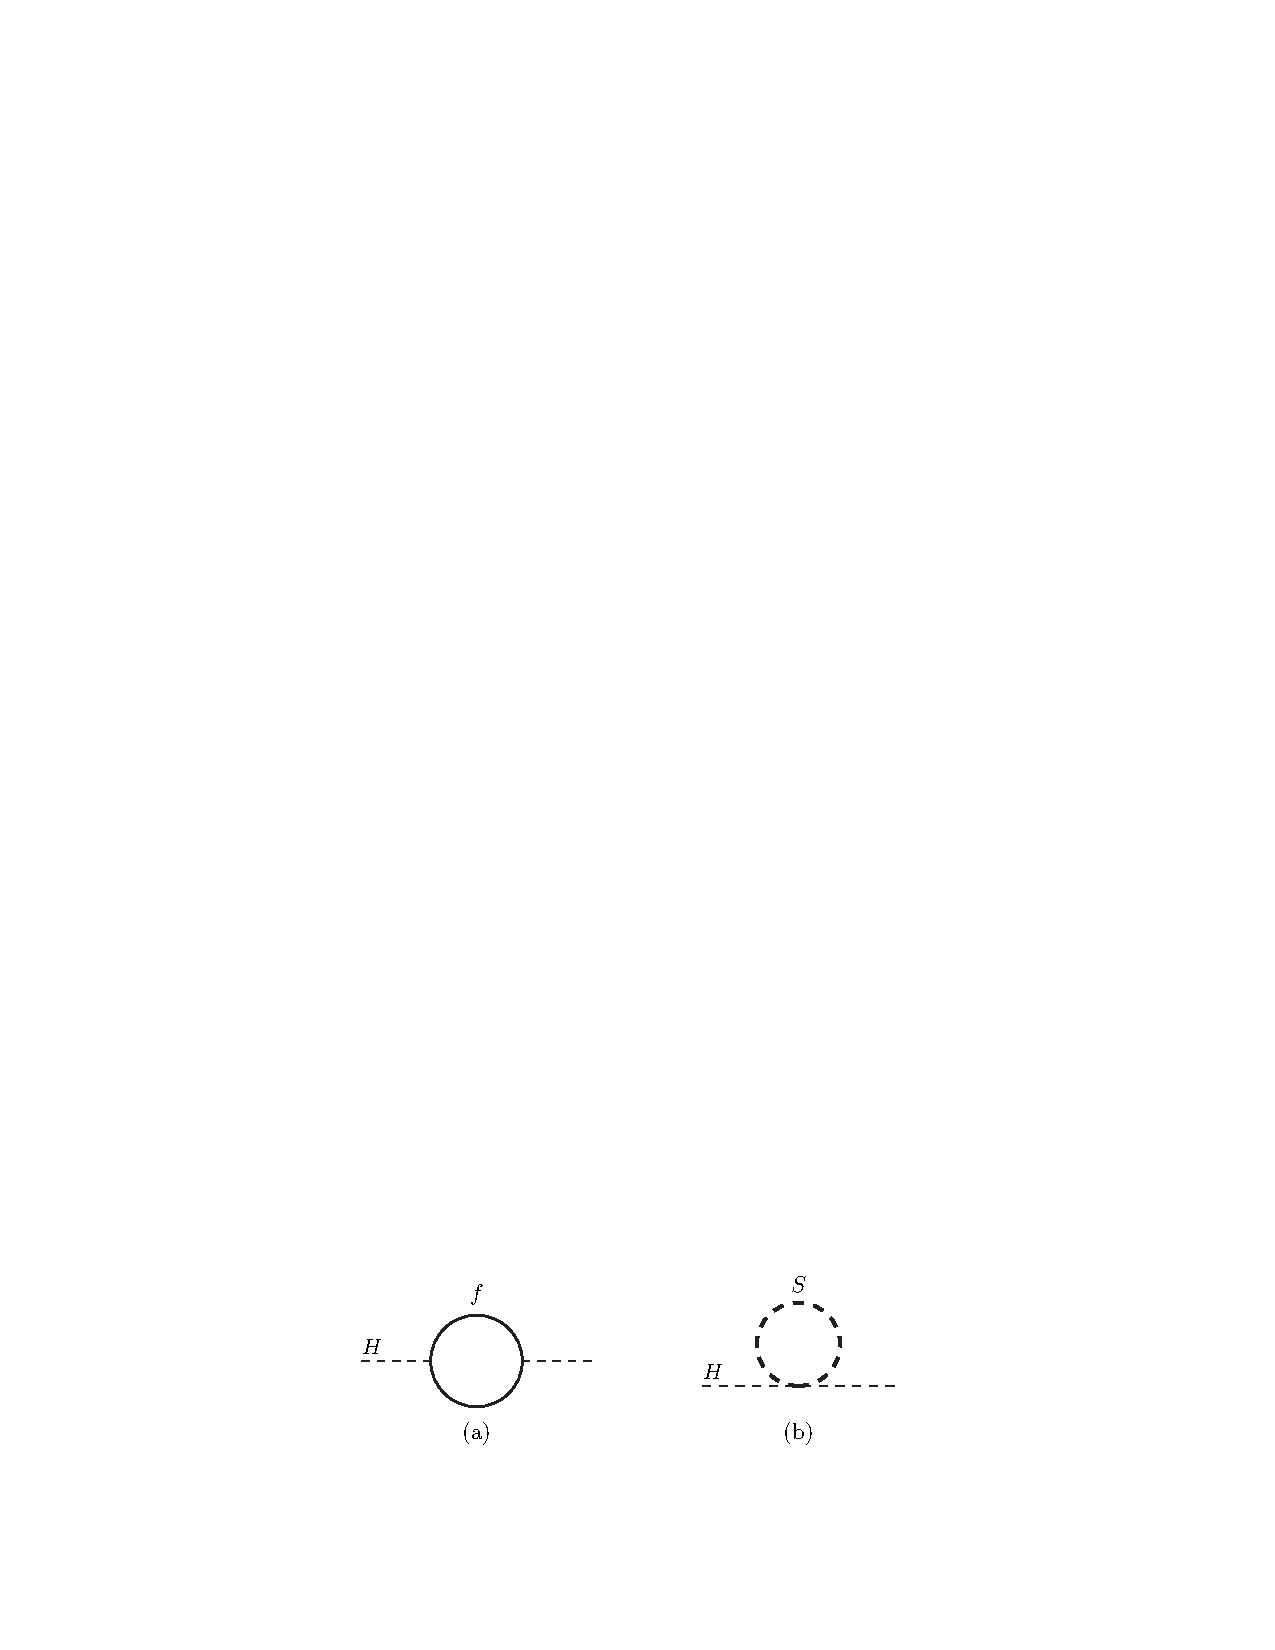
\includegraphics[width=0.7\textwidth]{Figures/Theory/hierarchyLoop.pdf}
    \caption{One-loop quantum corrections to the Higgs mass parameter $\mu^2$ from a Dirac fermion $f$ (left) and a scalar $S$ (right).
    Reprinted from Reference~\cite{SUSYprimer}.}
    \label{fig:hierarchy}
\end{figure*}


Even if it does not couple directly to the Higgs, any new particle would also contribute to $\mu^2$ at the two-loop level if it participates in the SM gauge interactions. For example, consider a heavy fermion $F$ with mass $m_F$ that only couples indirectly to the Higgs. Example two-loop Feynman diagrams are shown in 
\ref{fig:hierarchyFermi}. For such a fermion, the quantum corrections will be given by
\begin{equation}
\Delta\mu^2 = C(\frac{g^2}{16\pi^2})^2 [a \Lambda^2_\mathrm{UV} + 24m_F^2 \ln(\Lambda_\mathrm{UV}/m_F) +...]
\label{equ:corrTwoLoopFermi}
\end{equation}
where the constant $C$ represents several group theory factors, $a$ depends on the renormalization method, and $g$ is the gauge coupling. 

\begin{figure*}[htbp]
    \centering
    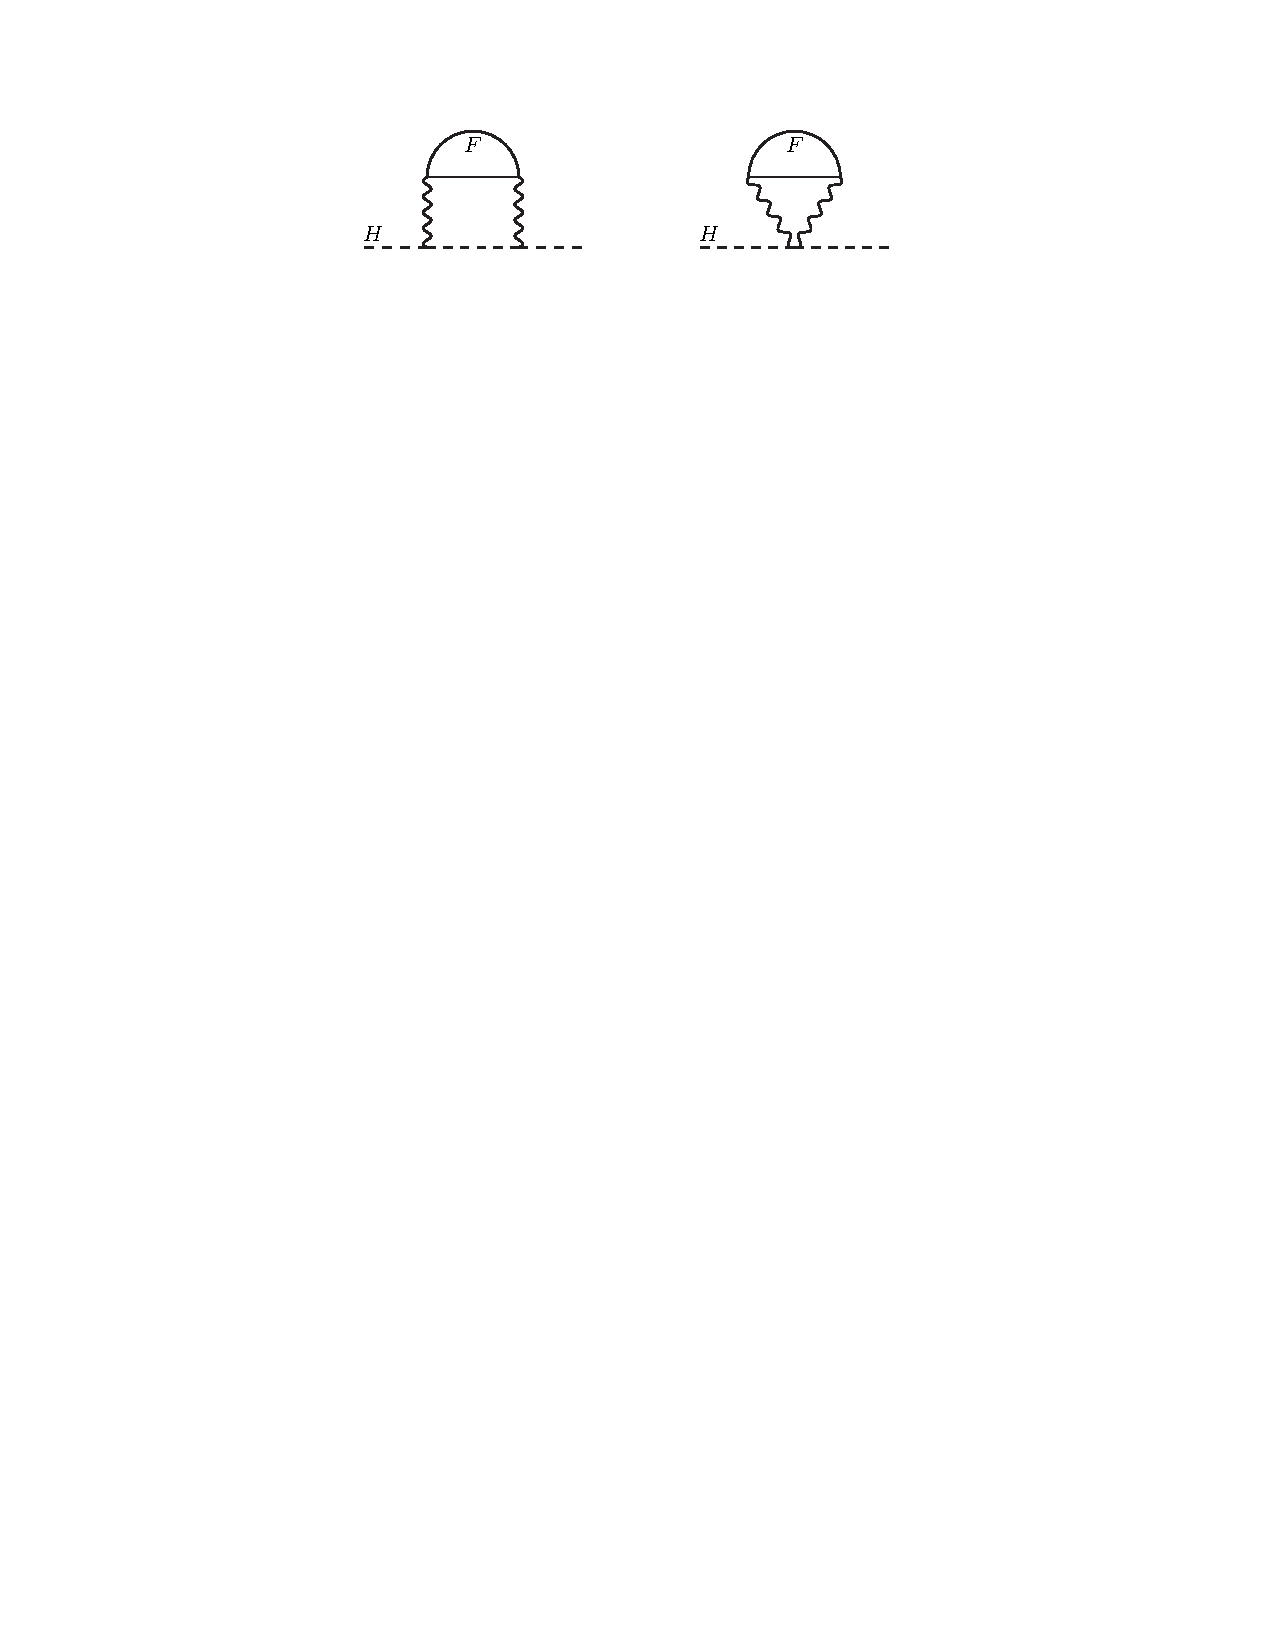
\includegraphics[width=0.7\textwidth]{Figures/Theory/hierarchyLoopFermi.pdf}
    \caption{Two-loop quantum corrections to the Higgs mass parameter $\mu^2$ from a fermion $F$ that couples indirectly to the Higgs through gauge interactions.
    Reprinted from Reference~\cite{SUSYprimer}.}
    \label{fig:hierarchyFermi}
\end{figure*}

The root of the hierarchy problem is the presence of $\Lambda^2_\mathrm{UV}$ in both Equations~\ref{equ:corrFermion} and \ref{equ:corrTwoLoopFermi}. If $\Lambda^2_\mathrm{UV}$ is near the Planck scale ($M_P = 2 \times 10^{18}$ GeV), then the corrections to $\mu^2$ are an unbelievable 30 orders of magnitude above its observed value. If we use dimensional regularization, it is possible to get rid of the $\Lambda^2_\mathrm{UV}$ terms in Equations~\ref{equ:corrFermion} and \ref{equ:corrTwoLoopFermi}, but the term proportional to $m_F^2$ remains \cite{SUSYprimer}. Since it seems incredibly unlikely that there are no new particles to be found in the 16 orders of magnitude between the electroweak and Planck scales, there is a tension between the experimentally-preferred and the theoretically-preferred values.

As will be discussed next, this observation has motivated many proposed extensions to the standard model, including supersymmetry.

%%%%%%%%%%%%%%%%%%%%%%%%%%%%%%%%%%%%%%%

%12 vector fields (spin 1)- gauge fields of the SU(3) x SU(2) x U(1)
%45 Weyl fermion fields: [21 Dirac spinors  (3 colors x 6 quarks) + 3 charged leptons] x2 to get to  weyl+ 3 neutrinos
%complex doublet H of scalar fields

%Left-handed Weyl components of quark Dirac spinors form 9 doublets of $SU(2)_W$ (3 flavor doublets per 3 color)
%Right-handed Weyl components of quark Dirac spinors are 18 $SU(2)_W$ singlets. Weak interactions can break parity

%Left-handed leptons form 3 $SU(2)_W$ doublets 
%right-handed leptons form singlets. If right-handed neutrinos exist, they are sterile and we have no evidence (can't have evidence?) for them
%Dirac spinor $\Psi$ and conjugate $\bar{\Psi}$ are equivalent to two left-handed Weyl spinors ($\chi$ and $\tilde{\chi}$)
%and their right-handed conjugates ($\chi^\dagger$ and $\tilde{\chi}^\dagger$).Tilde = anti


%http://bolvan.ph.utexas.edu/~vadim/Classes/2011f/SM.pdf

\section{Supersymmetry}
\label{sec:SUSY}

Supersymmetry (SUSY) is a particularly beautiful theoretical framework that addresses several of the standard model limitations described above. A ``supersymmetry" is a symmetry relating bosons and fermions. The supersymmetric operator $Q$ turns a bosonic state into a fermionic state:
\begin{equation}
Q|\mathrm{boson}\rangle = |\mathrm{fermion}\rangle, \hspace{35pt} Q|\mathrm{fermion}\rangle = |\mathrm{boson}\rangle
\label{equ:SUSYdef}
\end{equation}

The immediate consequence is that the number of elementary particles is at least double that in the standard model. For each SM boson, there will be a fermion ``superpartner" and vice versa. The deeper implications of Equation~\ref{equ:SUSYdef}, however, have many interesting effects, some of which 
provide attractive solutions to the issues with the SM listed above.

\subsection{Supersymmetric solution to the hierarchy problem}
\label{sec:SUSYhierarchy}

The key to solving the hierarchy problem with supersymmetry appears if we consider a heavy complex scalar $S$ with mass $m_S$. If the interaction term between $S$ and $H$ in the Lagrangian is $-\lambda_S|H|^2|S|^2$, then diagrams such as those in Figure~\ref{fig:hierarchy}b give rise to the following quantum corrections:
\begin{equation}
\Delta\mu^2 = -\frac{\lambda_S^2}{16\pi^2} [ \Lambda^2_\mathrm{UV} - 2 m_S^2 \ln{\Lambda_\mathrm{UV} / m_S) }+ ... ]
\label{equ:corrScalar}
\end{equation}

Upon close inspection of Equations~\ref{equ:corrFermion} and \ref{equ:corrScalar}, it becomes clear that if
there are two complex scalars per fermion that satisfy $\lambda_S = |\lambda_f|^2$, then the contributions to $\mu^2$ proportional to $ \Lambda^2_\mathrm{UV}$ cancel exactly. 
Less obvious is whether the contributions from diagrams with more loops also cancel. The good news is that it can be shown that 
the contributions to $\mu^2$ cancel to all orders in a supersymmetric theory. Any new particles, even extremely massive ones, would be
accompanied by their superpartners and $\mu^2$ would remain unaffected.

%%%%%%%%%%%%%%%%%%%%%%%%%%%%%%%%%%%%%%%
%%%%%%%%%%%%%%%%%%%%%%%%%%%%%%%%%%%%%%%
%%%%%%%%%%%%%%%%%%%%%%%%%%%%%%%%%%%%%%%

\subsection{Particles in minimal SUSY models}
\label{sec:SUSYparticles}
In a supersymmetric theory, the SM particles shown in Tables~\ref{tab:fermions} and \ref{tab:bosons} must be arranged into ``supermultiplets" containing the SM fermions and bosons and their superpartners. There must be an equal number of bosonic and fermionic degrees of freedom in each supermultiplet ($n_b$ and $n_f$, respectively). The SM particles fall into two types of supermultiplets:
\begin{itemize}
\item The standard model fermions belong to \textbf{chiral supermultiplets}. Each chiral supermultiplet contains one Weyl fermion ($n_f = 2$) and a complex scalar field ($n_b = 2$).
\item The spin-1 gauge bosons belong to \textbf{gauge supermultiplets}. Before EWSB, the gauge bosons are massless and have $n_b = 2$. Their superpartners are massless spin-1/2 Weyl fermions with $n_f = 2$. 
\end{itemize}

The Minimal Supersymmetric Standard Model (MSSM) is the most basic SM extension that incorporates SUSY. Table~\ref{tab:SUSY_fermions} lists the chiral supermultiplets in the MSSM, and the gauge supermultiplets are listed in Table~\ref{tab:SUSY_bosons}. Note that all particles in a supermultiplet are in the same representation of $G_{SM}$. 

There must be two Higgs chiral supermultiplets in the MSSM to avoid gauge anomalies in the electroweak gauge symmetry, one with hypercharge $\Upsilon = 1/2$ and one with $\Upsilon = -1/2$. The $\Upsilon = 1/2$ chiral supermultiplet $H_u$ has the Yukawa couplings necessary to give masses to the up-type quarks, and the Yukawa couplings of the $\Upsilon = -1/2$ chiral supermultiplet $H_d$ give masses to the down-type quarks. The 125 GeV standard model Higgs boson is a linear combination of $H_u^0$ and $H_d^0$.

%popular proposed SM extensions to solve the hierarchy problem. 
%%%%%%%%%%%%%%%%%%%%%%%%%%%%%%%%%%%%%%%

\begin{table}[ht]
    \caption{CHIRAL SUPERMULTIPLETS IN MSSM}
    \centering
    \begin{tabular}{|c|c|c|c|c|}
    \hline
    \hline
    \multicolumn{2}{|c|}{Names} & Spin 0 & Spin 1/2 &$SU(3)_C,~SU(2)_L,~U(1)_\Upsilon $\\
  	  \hline
           \hline    
squarks, quarks  & Q & ($\tilde{u}_L~\tilde{d}_L$) & ($u_L~d_L$)  & (\textbf{3}, \textbf{2}, $\frac{1}{6}$) \\
(3 families) & $\bar{u}$ & $\tilde{u}_R^\ast$ & $u_R^\dagger$ & ($\bar{\textbf{3}}$, \textbf{1}, $-\frac{2}{3}$) \\
                   & $\bar{d}$ & $\tilde{d}_R^*$     & $d_R^\dagger$ & ($\bar{\textbf{3}}$, \textbf{1}, $\frac{1}{3}$) \\
                   \hline
sleptons, leptons  & $L$ & ($\tilde{\nu}~\tilde{e}_L$) & ($\nu~e_L$)      &  (\textbf{1}, \textbf{2}, $-\frac{1}{2}$) \\
(3 families) & $\bar{e}$ & $\tilde{e}_R^\ast$  & $e_R^\dagger$ &  (\textbf{1}, \textbf{1}, 1) \\
\hline
Higgs, higgsinos & $H_u$  & ($H_u^+ ~ H_u^0$) & ($\tilde{H}_u^+ ~ \tilde{H}_u^0$) & ($\textbf{1}$, \textbf{2}, $+\frac{1}{2}$) \\
                           & $H_d$  & ($H_d^0 ~ H_d^-$) & ($\tilde{H}_d^0 ~ \tilde{H}_d^-$) & ($\textbf{1}$, \textbf{2}, $-\frac{1}{2}$) \\
           \hline
           \hline
    \end{tabular}
    \label{tab:SUSY_fermions}
    \justify{List of chiral supermultiplets in the MSSM. Reprinted from Reference~\cite{SUSYprimer}.}
\end{table}
%%%%%%%%%%%%%%%%%%%%%%%%%%%%%%%%%%%%%%%

\begin{table}[ht]
    \caption{GAUGE SUPERMULTIPLETS IN THE MSSM}
    \centering
    \begin{tabular}{|c|c|c|c|c|}
    \hline
    \hline
    Names & Spin 1/2 & Spin 1 &$SU(3)_C,~SU(2)_L,~U(1)_\Upsilon $\\
  	  \hline
           \hline    
gluino, gluon & $\tilde{g}$ & $g$   & (\textbf{8}, \textbf{1}, 0) \\
\hline
wino, $W$ bosons & $\widetilde{W}^\pm,~\widetilde{W}^0$ & $W^\pm,~W^0$ & (\textbf{1}, \textbf{3}, 0) \\
\hline
bino, $B$ boson & $\widetilde{B}^0$ & $B^0$ & (\textbf{1}, \textbf{1}, 0) \\
           \hline
           \hline
    \end{tabular}
    \label{tab:SUSY_bosons}
    \justify{List of gauge supermultiplets in the MSSM. Reprinted from Reference~\cite{SUSYprimer}.}
\end{table}

The names of the MSSM superpartners are very creatively derived from their SM counterparts. For fermions, the SM names are prefixed with ``s" to get the superpartner name: electrons to selectrons, quarks to squarks, etc. For bosons, the suffix ``ino" is added: $W$ to wino, gauge boson to gaugino, etc. The symbols for supersymmetric particles are given simply by adding a tilde to the SM symbol. For example, $\tilde{e}$ is the symbol for the selectron.

After EWSB, the neutral higgsinos ($\widetilde{H}_u^0$ and $\widetilde{H}_d^0$) and the neutral electroweak gauginos ($\widetilde{W}_0$ and $\widetilde{B}_0$) form four mass eigenstates known as neutralinos $\widetilde{\chi}^0$. The charged higgsinos ($\widetilde{H}_u^+$ and $\widetilde{H}_d^-$) and charged winos ($\widetilde{W}^\pm$) form four mass eigenstates known as charginos $\widetilde{\chi}^\pm$. 


%%%%%%%%%%%%%%%%%%%%%%%%%%%%%%%%%%%%%%%
%%%%%%%%%%%%%%%%%%%%%%%%%%%%%%%%%%%%%%%

\subsection{$R$-parity}
\label{sec:Rparity}
Phenomenologically, an important feature of many SUSY models is $R$-parity conservation.
$R$-parity is a new symmetry introduced in the MSSM to get rid of interactions that violate lepton number $L$
or baryon number $B$. 
Experimentally, we know that if $B$- and $L$-violating processes occur, they must be extremely suppressed. 
In particular, the lifetime of the proton must be greater than $10^{32}$ years \cite{SUSYprimer}. 
Without $R$-parity conservation, however, it is possible to write down terms in the MSSM Lagrangian 
that would allow the proton to decay to $e^+\pi^0$ or other 
lepton + meson combinations with a lifetime of less than one second.

$R$-parity (also known as matter parity) is a conserved quantum number:
\begin{equation}
P_R = (-1)^{3(B-L)+2s}
\end{equation}
where $s$ is the spin of the particle. All terms in the Lagrangian are required to satisfy $\prod P_{R} = +1$, where the product
is over all fields in the term. The SM particles and the Higgs bosons have $P_R = +1$, and
all SUSY particles---squarks, sleptons, gauginos, and higgsinos---have $P_R = -1$.

Most models of SUSY, including those explored in this analysis, assume $R$-parity conservation.
One immediate consequence is that each vertex must have an even number of supersymmetric particles (``sparticles").
In a collider experiment 
%where there are no SUSY particles initially, 
this means that sparticles must be pair-produced.
Additionally, $R$-parity conservation implies that the lightest supersymmetric particle (LSP) must be absolutely stable.
All other sparticles will eventually decay to the LSP. From the high energy experimentalist's point of view, this means that the 
primary signature of SUSY production in colliders will be significant missing transverse momentum. 
From the cosmologist's point of view, this means that the LSP, if electrically neutral, 
is a potential dark matter candidate

%%%%%%%%%%%%%%%%%%%%%%%%%%%%%%%%%%%%%%%
%%%%%%%%%%%%%%%%%%%%%%%%%%%%%%%%%%%%%%%
%%%%%%%%%%%%%%%%%%%%%%%%%%%%%%%%%%%%%%%
%%%%%%%%%%%%%%%%%%%%%%%%%%%%%%%%%%%%%%%
%%%%%%%%%%%%%%%%%%%%%%%%%%%%%%%%%%%%%%%
%cite http://pdg.lbl.gov/2015/reviews/rpp2015-rev-susy-2-experiment.pdf

\section{Gauge-mediated supersymmetry breaking}
\label{sec:gmsb}

So far no SUSY particles have been observed. If SUSY were an unbroken symmetry, then the masses of the superpartners
would be the same as their SM counterparts. The lack of experimental detection means that SUSY must be a broken symmetry.
Theorists have come up with many different mechanisms by which SUSY can be broken. 
The SUSY breaking mechanism and the SUSY breaking scale 
determine the phenomenology of the model, including the SUSY particle masses and their allowed decay modes.

In gauge-mediated supersymmetry breaking (GMSB), SUSY is spontaneously broken in a ``hidden" sector that is decoupled from the SM interactions. 
New chiral supermultiplets known as messengers interact with the hidden sector and 
also interact with the ``visible" sector (ie, SM particles and their superpartners) through the normal
SM gauge interactions. The messengers are said to communicate between the two sectors and relay the information about the SUSY breaking.
From the lack of experimental observation, we know that the masses of the messenger particles must be very high. 

One of the nice features of GMSB is that the flavor symmetry of the SM is preserved, because the gauge interactions are flavor-blind. 
The messengers give mass to the sparticles through loop diagrams such as those shown in 
Figure~\ref{fig:GMSBgaugino} for gauginos and Figure~\ref{fig:GMSBscalars} for the squarks and sleptons. 

\begin{figure*}[htbp]
    \centering
    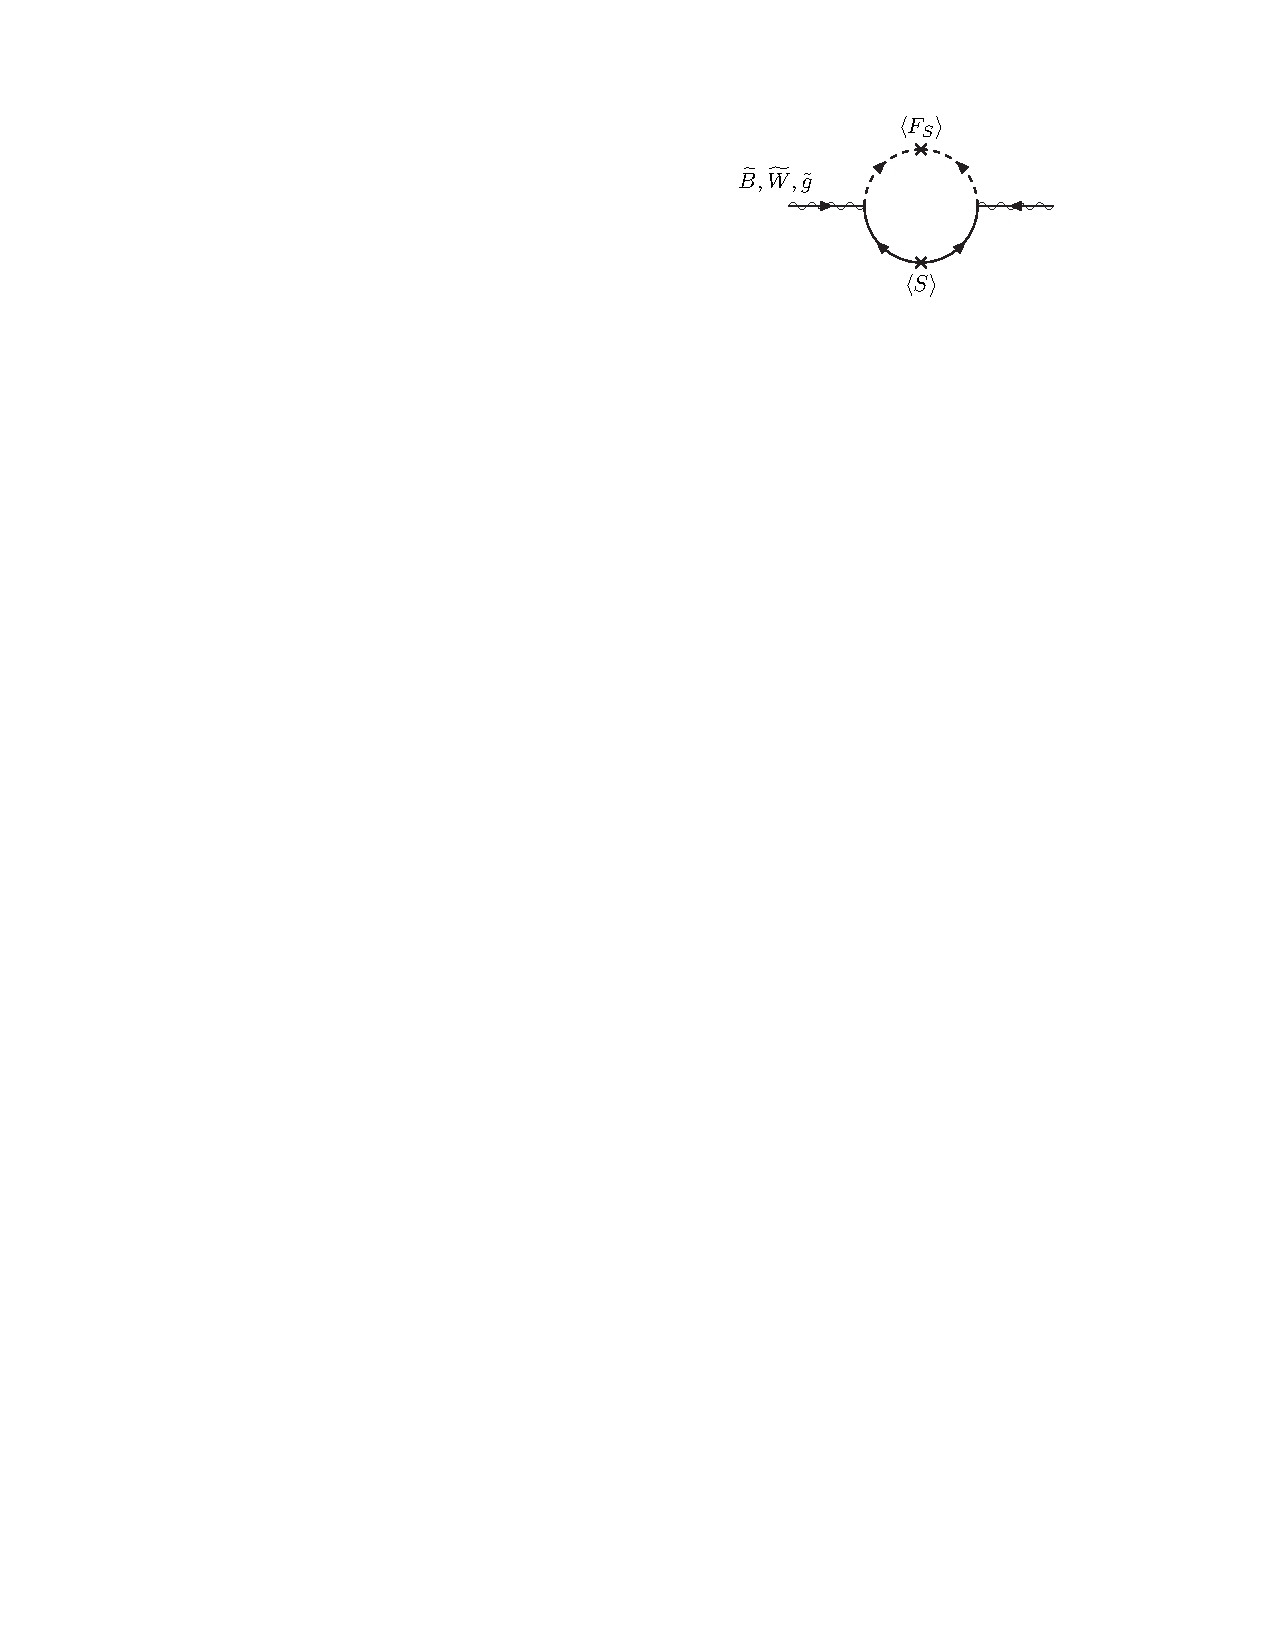
\includegraphics[width=0.4\textwidth]{Figures/Theory/GMSBgaugino.pdf}
    \caption{Feynman diagram illustrating how the messenger particles in SUSY models
    with general gauge mediation give rise to mass terms for the MSSM gauginos. 
    Wavy lines superimposed on straight lines represent the gauginos, and 
    $\langle F_S \rangle$ and $\langle S \rangle$ represent messenger particles.
    Reprinted from Reference~\cite{SUSYprimer}.}
    \label{fig:GMSBgaugino}
\end{figure*}

\begin{figure*}[htbp]
    \centering
        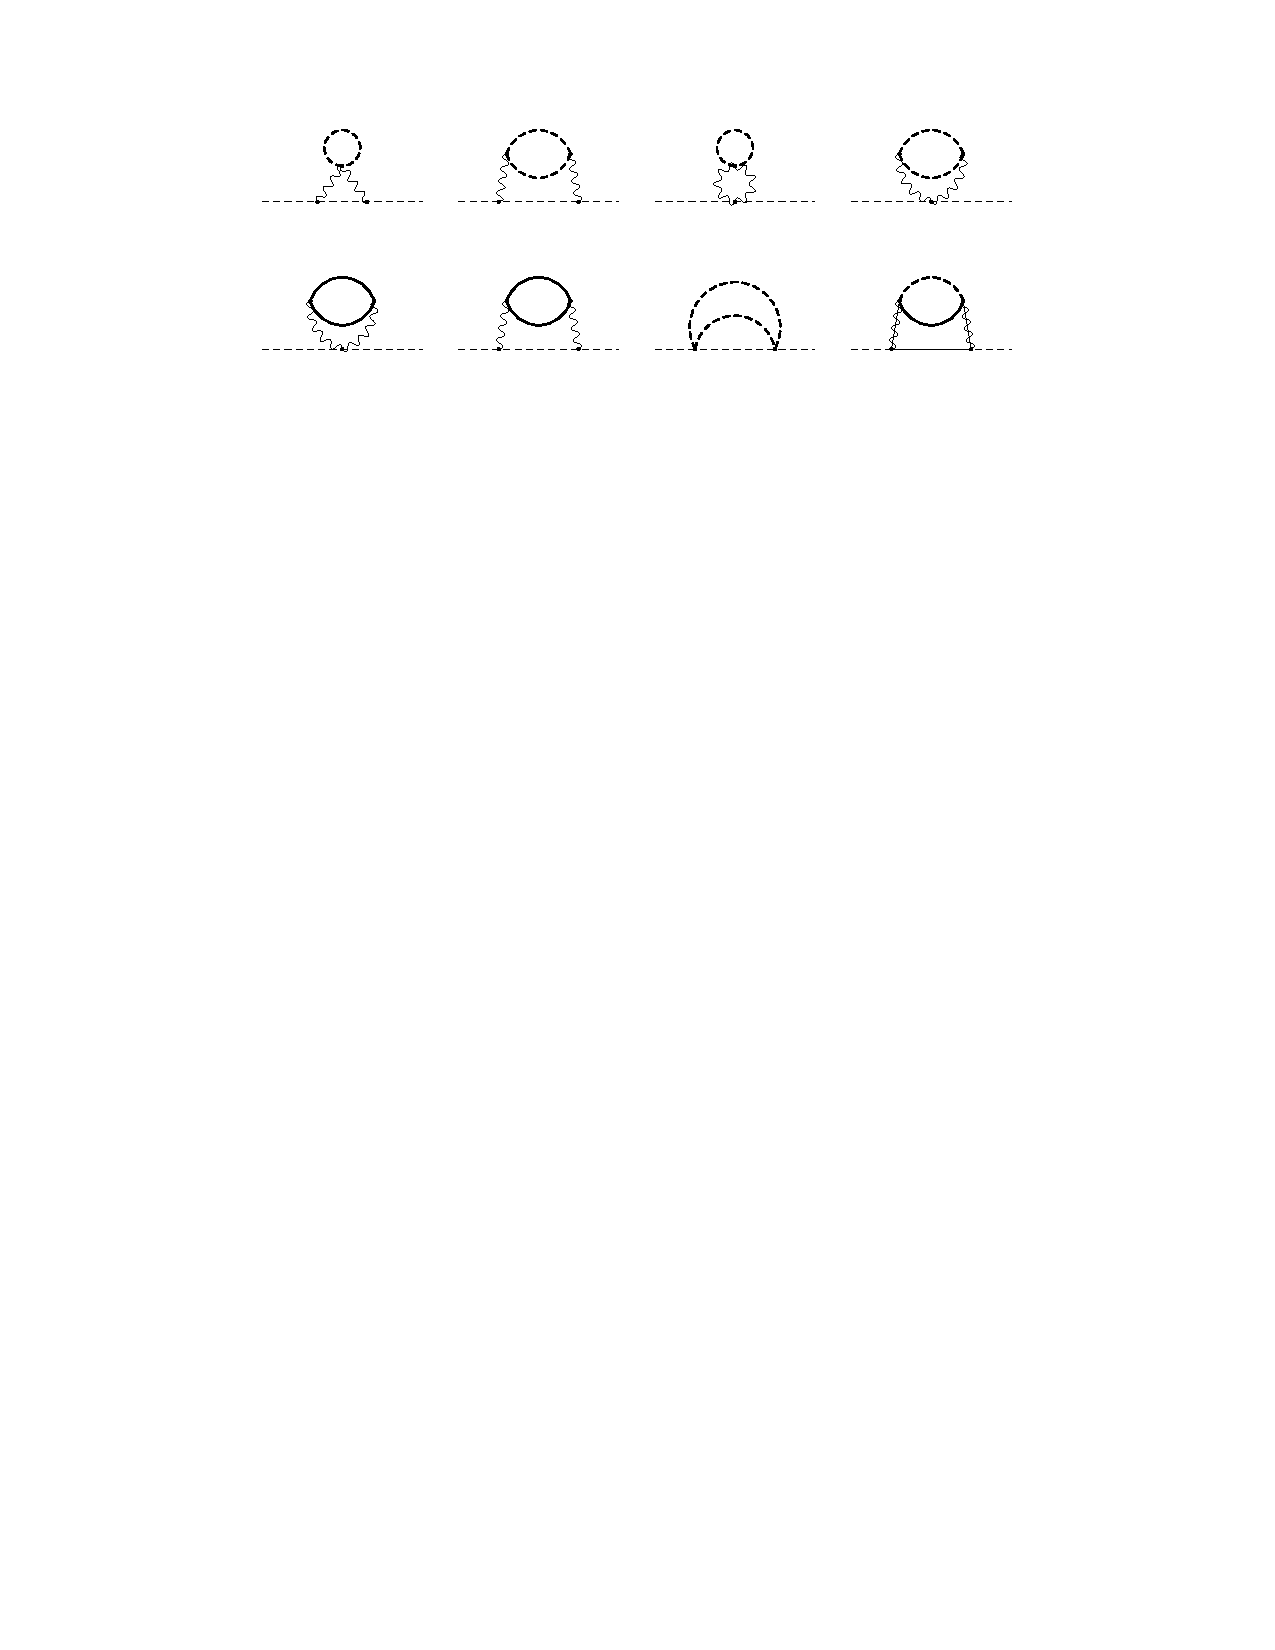
\includegraphics[width=\textwidth]{Figures/Theory/GMSBscalar.pdf}
    \caption{Example Feynman diagrams illustrating how the messenger particles in SUSY models
    with general gauge mediation give rise to mass terms for 
    the MSSM scalars. Wavy lines superimposed on straight lines represent the MSSM gauginos, 
    dotted lines represent the MSSM scalars, wavy lines represent the SM gauge bosons, heavy dashed lines
    represent messenger scalars, and solid lines represent messenger fermions.
    Reprinted from Reference~\cite{SUSYprimer}.}
    \label{fig:GMSBscalars}
\end{figure*}

GMSB usually refers to the minimal version of the theory, where the hidden sector includes a single field $S$ that is a singlet under $G_{SM}$. 
The more general framework is referred to as general gauge mediation (GGM). 

The GGM phenomenology is independent from the exact SUSY-breaking mechanism in the hidden sector. In particular, 
in all GGM models, the lightest supersymmetric particle is the gravitino \gravitino, the superpartner of the graviton. 
The graviton is a spin-2 particle, which means the graviton and gravitino can not belong to either the chiral or gauge supermultiplets described in Section~\ref{sec:SUSYparticles}. Instead, the gravitino is a spin-3/2 particle.

In GGM, the gravitino must be significantly lighter than all other sparticles, on the order of eV to keV. The gravitino only interacts
gravitationally with SM particles and therefore escapes the detector without depositing its energy. This causes 
an imbalance in the reconstructed momentum in the transverse plane of the detector and is referred to as missing 
transverse momentum $\vec{\pt}^{\mathrm{miss}}$. The magnitude of $\vec{\pt}^{\mathrm{miss}}$ is called the
missing transverse energy, or \ETmiss.

The next-to-lightest supersymmetric particle (NLSP) is either the lightest chargino or the lightest neutralino.
In this analysis, we will only consider models where the NLSP is the neutralino. We further constrain 
ourselves to models where the neutralino decays promptly. In general, the allowed neutralino decays are
$\neutralino \rightarrow \gamma\gravitino$, $\neutralino \rightarrow H\gravitino$, or $\neutralino \rightarrow Z\gravitino$,
but the first case normally dominates. We will assume 100\% branching fraction of $\neutralino \rightarrow \gamma\gravitino$
for the interpretation of our results.

If we assume $R$-parity conservation, then sparticles must be pair-produced and eventually decay to a gravitino. 
In a $p$-$p$ collider such as the LHC, the dominant production modes for SUSY particles are either gluino pair production
or squark pair production. Example decay chains are shown in Figure~\ref{fig:gluinoSquarkDecay1}. The final state 
signature is characterized by two photons and significant \ETmiss.

\begin{figure*}[htbp]
    \centering
    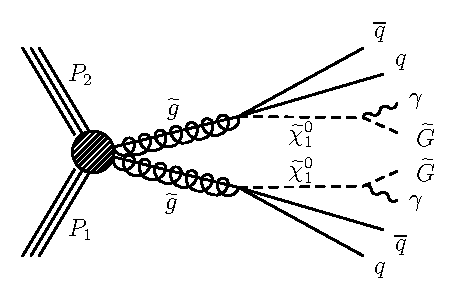
\includegraphics[width=0.45\textwidth]{Figures/Results/gluinoDecay.pdf}
    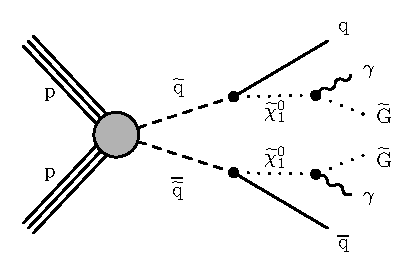
\includegraphics[width=0.45\textwidth]{Figures/Results/squarkDecay.pdf}
    \caption{Diagrams showing the production of signal events in the collision
        of two protons with four momenta ${P}_{1}$ and ${P}_{2}$. 
        The diagram on the left illustrates the decay chain for gluino pair production, and 
        the diagram on the right illustrates it for squark pair production. In both cases, 
        two neutralinos \neutralino are produced that each subsequently decay to a photon $\gamma$~and a gravitino \gravitino.
        In the diagram on the right, we do not distinguish between squarks and
        antisquarks.}
    \label{fig:gluinoSquarkDecay1}
\end{figure*}

\section{Experimental bounds on supersymmetry}
\label{sec:SUSYlimits}

So far, there has been no experimental evidence for supersymmetry. In the absence of evidence, limits
are placed on the allowed sparticle masses and SUSY process cross sections. 
During Run I of the LHC at CERN,
protons were collided at a center-of-mass energy $\sqrt{s} = 8$ TeV, setting a new record for high energy
collisions. No signs of physics beyond the standard model were observed. In 2015, the LHC successfully 
restarted at an even higher center-of-mass-energy, $\sqrt{s} = 13$ TeV. The increase in energy corresponded
to a large jump in discovery potential, but evidence for SUSY has still eluded us. 

Figure~\ref{fig:CMSexclusions} shows the excluded mass regions for EWK gauginos, squarks, and gluinos
from a wide variety of $\sqrt{s} = 13$ TeV CMS analyses \cite{SUSYtwiki}. Gluino masses below approximately 1800 GeV and 
squark masses below approximately 1000 GeV have been excluded at the 95\% confidence level. 
Figure~\ref{fig:CMSexclusions} does not contain any results interpreted in the context of GGM models.
The difference between the orange and blue bars illustrate the effect of nearly tripling the size of the
data set, from 12.9 \fbinv to 35.9 \fbinv. See Reference~\cite{pdgReview} for an full overview of SUSY 
limits from both colliders and precision measurements.

\begin{figure*}[htbp]
    \centering
    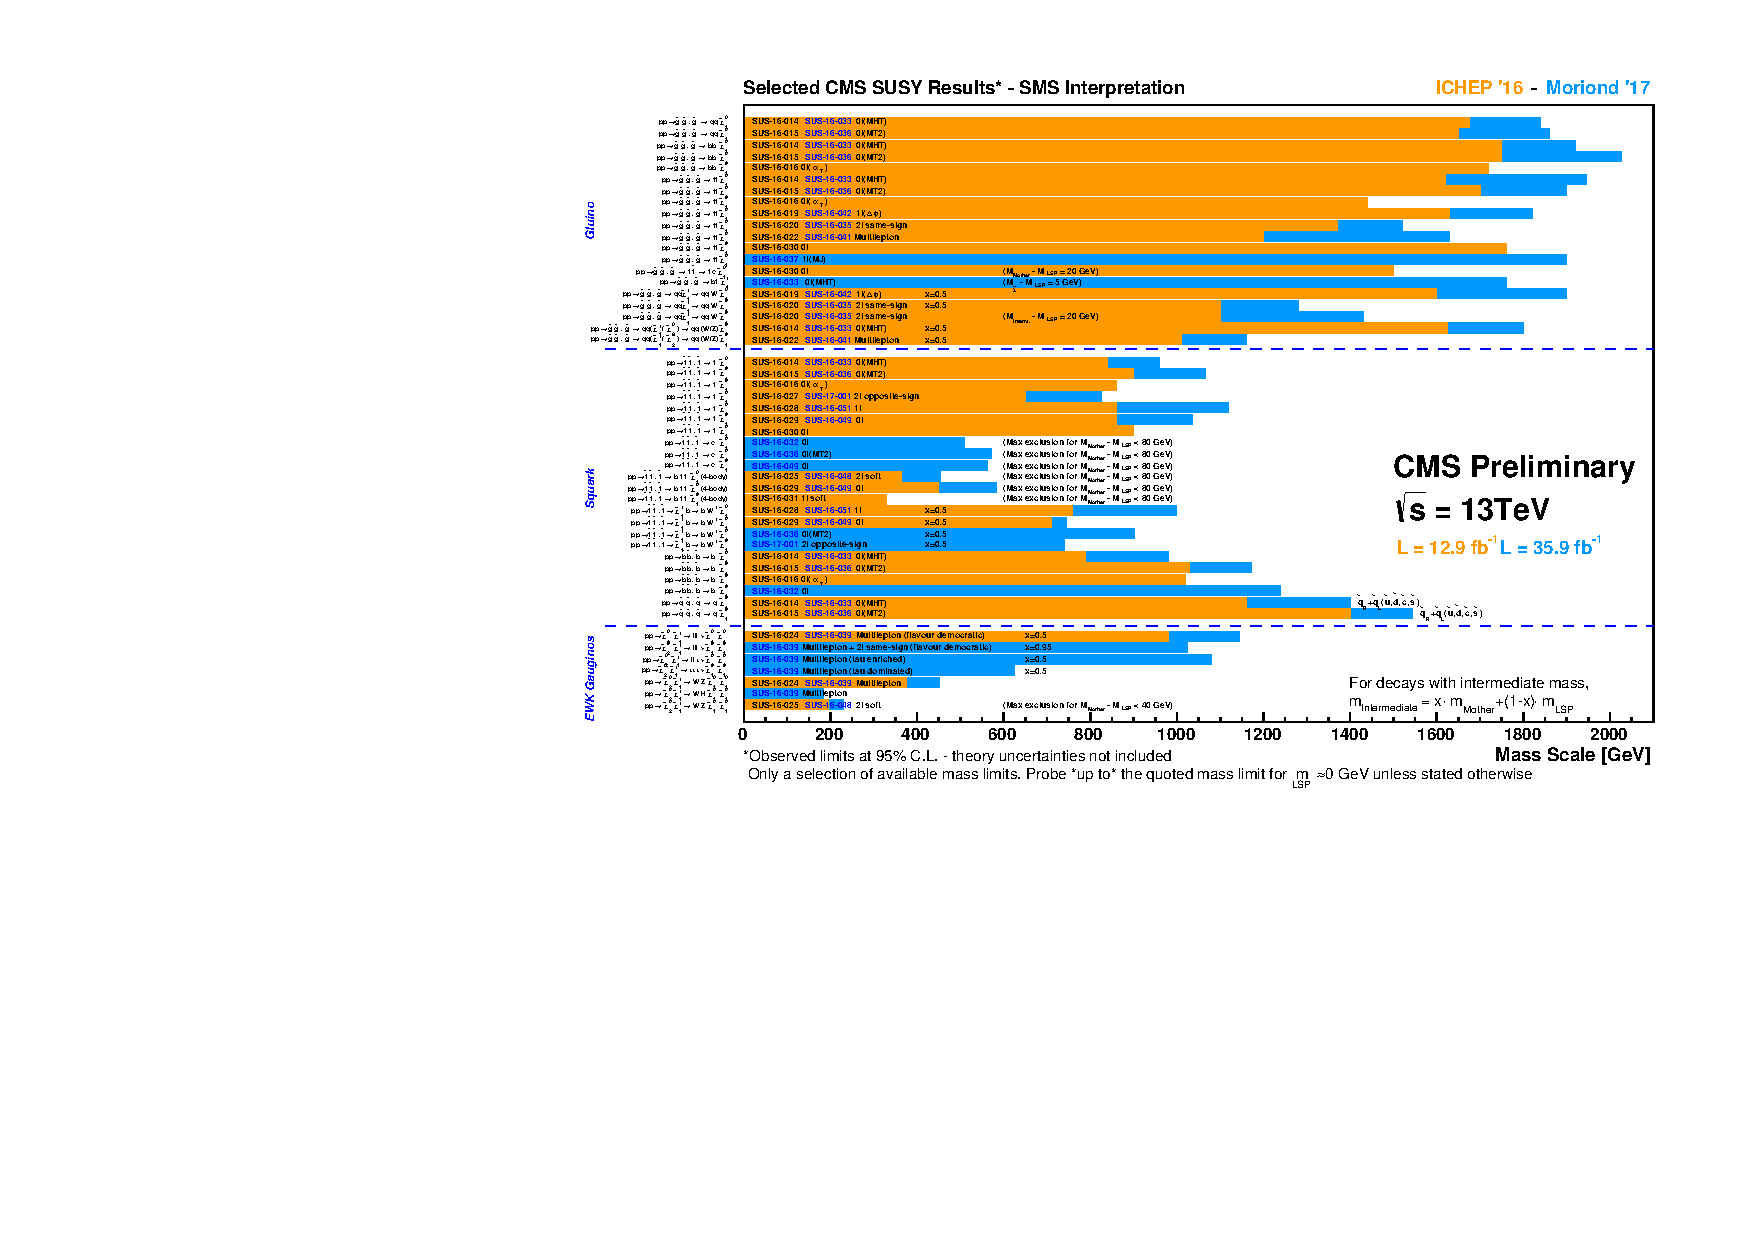
\includegraphics[angle=90,origin=c,width=.9\textwidth]{Figures/Theory/Moriond2017_BarPlot.pdf}
    \caption{ Excluded sparticle mass ranges for a selection of CMS results using the 2016 data set \cite{SUSYtwiki}.}
    \label{fig:CMSexclusions}
\end{figure*}

\subsection{Exclusion contours for GGM in the diphoton final state}
\label{sec:GMSBlimits}
Both CMS and ATLAS have published searches for GGM models in the diphoton final state, both at 8 TeV \cite{Aad:2015hea,Khachatryan:2015exa} and at 13 TeV \cite{ATLAS:2016aa,CMS:2015_anal}. Figure~\ref{fig:Limits2015CMS} shows the 95\% confidence level limits in the gluino versus neutralino and the squark versus neutralino mass planes using 2.3 \fbinv of 13 TeV data collected with the CMS detector in 2015. 
Gluino masses below 1.65 TeV and squark masses below 1.37 TeV have been excluded.
The simplified models used for the interpretation of results in Figure~\ref{fig:Limits2015CMS} will be described in more detail in Section~\ref{sec:SimplifiedModels}.

\begin{figure*}[h]
\begin{center}
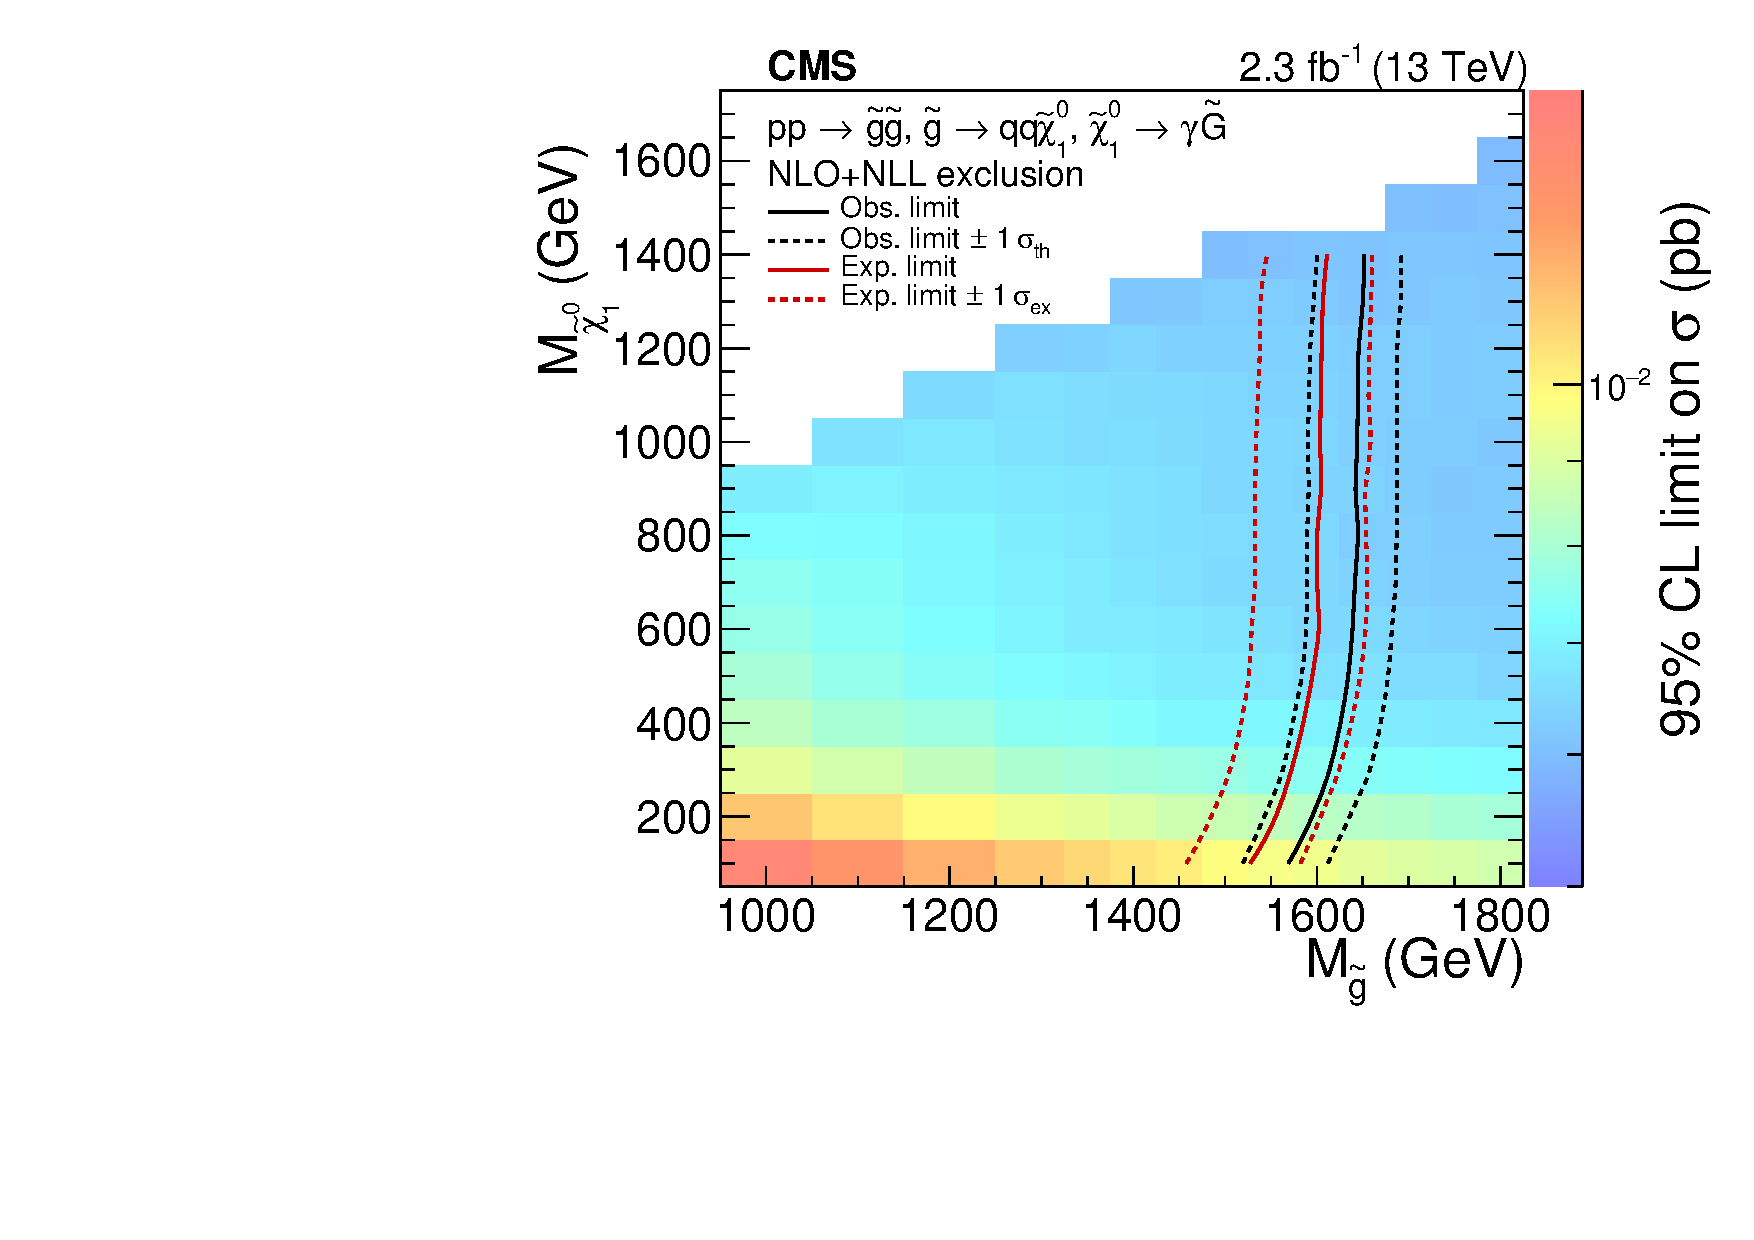
\includegraphics[width=0.49\textwidth]{Figures/Theory/2015gg.pdf}
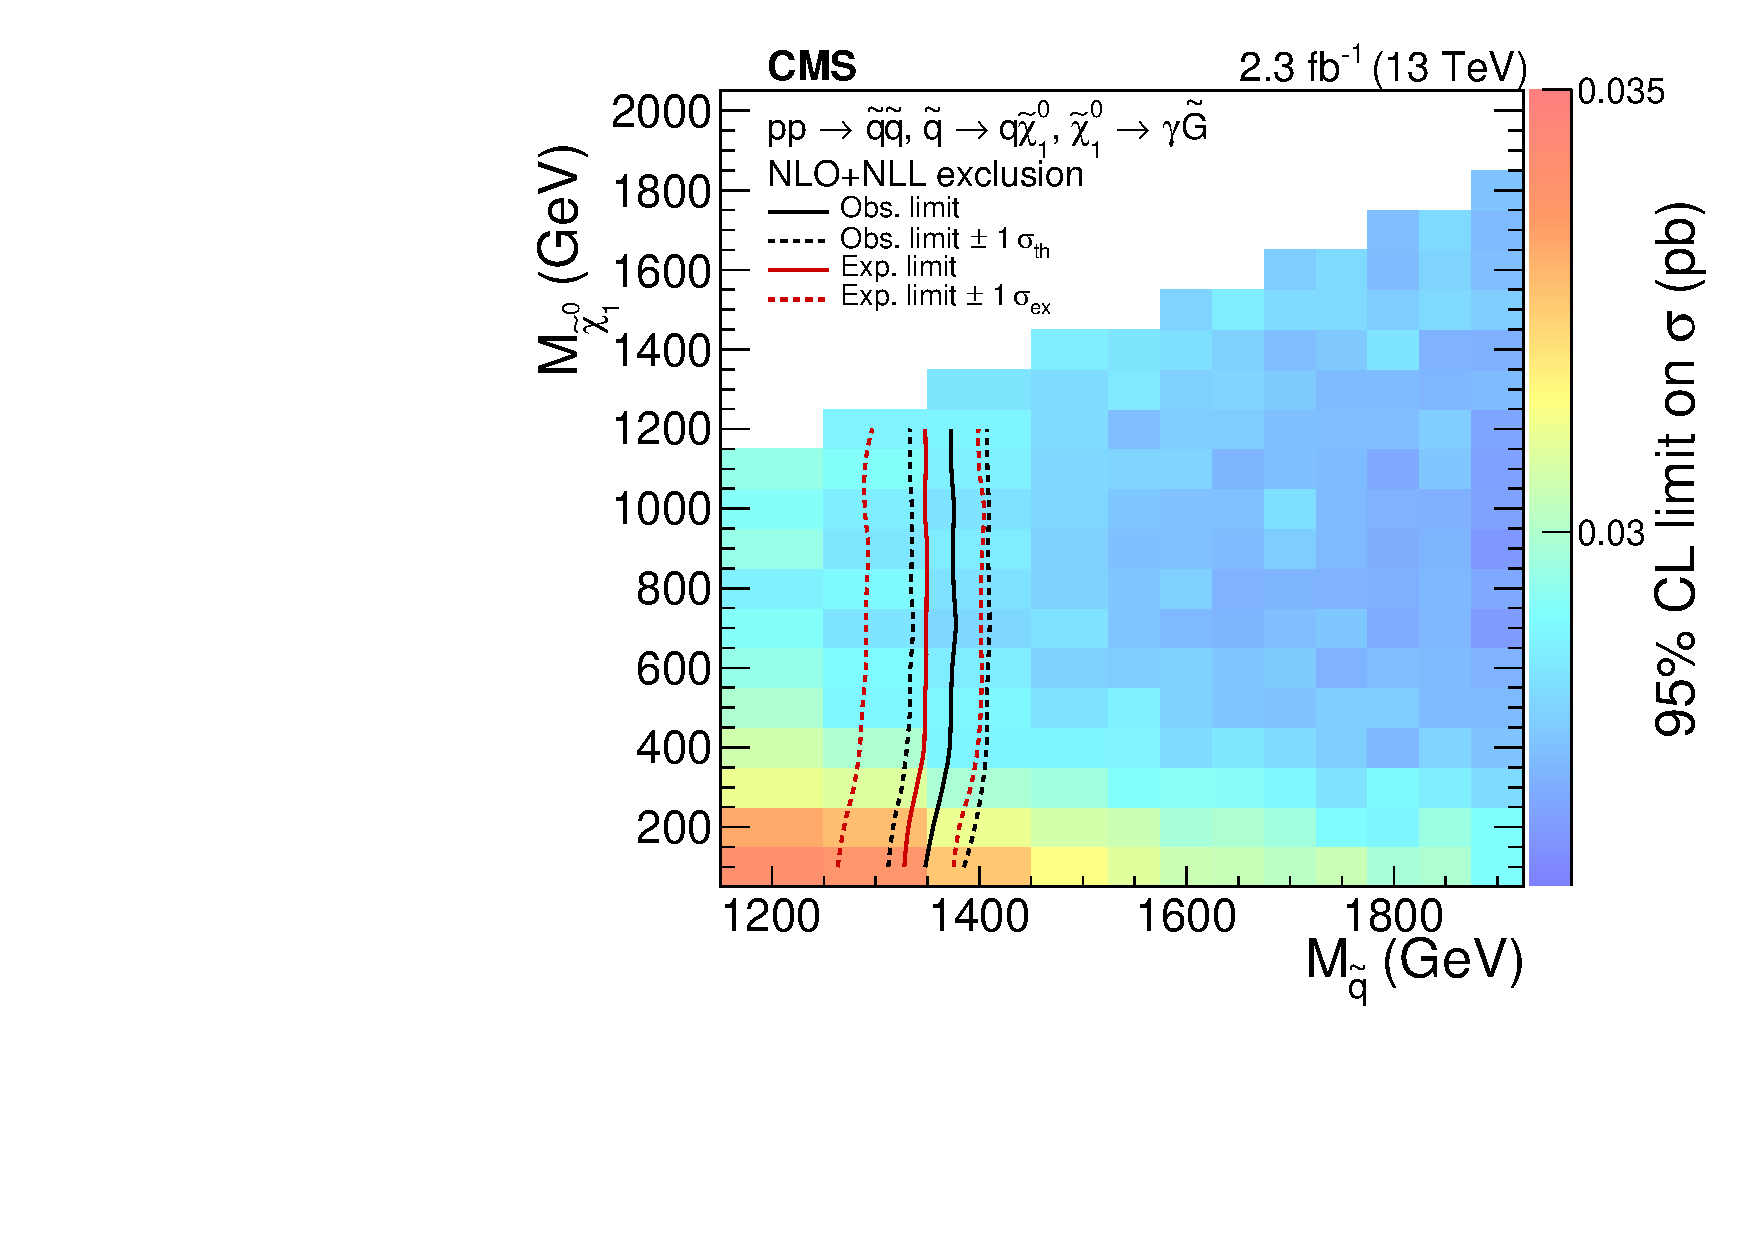
\includegraphics[width=0.49\textwidth]{Figures/Theory/2015qq.pdf}
\end{center}
    \caption{The 95\% CL upper limits on the gluino (left) and squark (right)
        pair production cross sections as a function of neutralino versus
	gluino or squark mass. The contours show the observed and median
        expected exclusions with their one
        standard deviation uncertainties. Reprinted from \cite{CMS:2015_anal}.}
    \label{fig:Limits2015CMS}
\end{figure*}

The 2015 ATLAS results are shown in Figure~\ref{fig:Limits2015ATLAS}. 
Limits were placed only on the masses of particles in a gluino pair production model. 
Gluino masses below 1.65 TeV were excluded at a 95\% confidence level.
The search strategy of the ATLAS analysis is similar to the CMS strategy. 
The primary difference is that ATLAS defines their signal regions so that the expected SM background is close to zero. 
This is the source of the asymmetric expected limits in Figure~\ref{fig:Limits2015ATLAS}.
The CMS methodology as applied to the 2016 data set is the main focus of this dissertation and 
will be described in detail, particularly in Chapter~\ref{chap:DataAnalysis}. 


\begin{figure*}[h]
\begin{center}
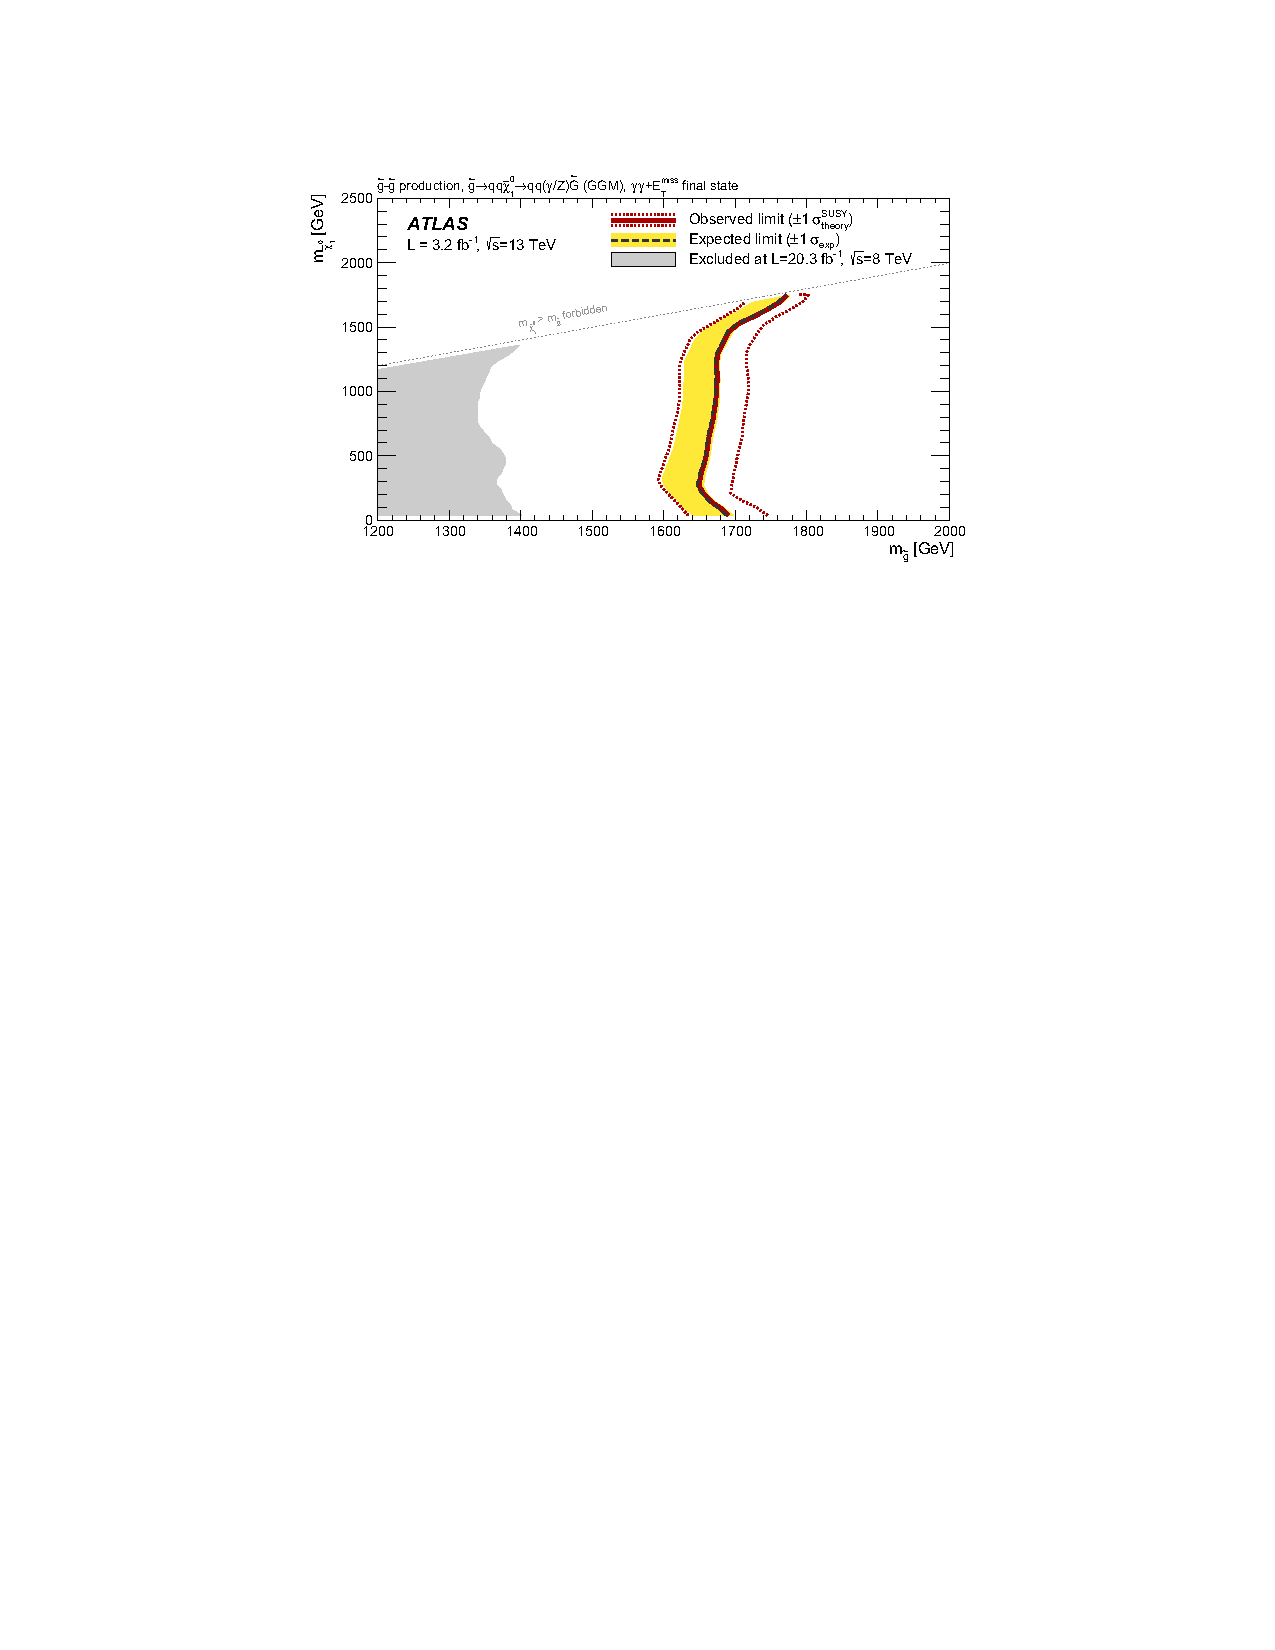
\includegraphics[width=0.8\textwidth]{Figures/Theory/2015ATLAS.pdf}
\end{center}
    \caption{95\% confidence level exclusion contours in the neutralino-gluino mass plane derived using 3.2 \fbinv of data collected with the ATLAS detector in 2015. The expected limits are shown in black, with a yellow band representing $\pm~1\sigma$, and the observed limits are shown in red, with dotted red lines representing $\pm~1\sigma$. The gray area is the region previously excluded by 8 TeV ATLAS analyses. Reprinted from \cite{ATLAS:2016aa}.}
    \label{fig:Limits2015ATLAS}
\end{figure*}


